\documentclass[hyperref, a4paper]{article}

\usepackage{geometry}
\usepackage{titling}
\usepackage{titlesec}
% No longer needed, since we will use enumitem package
% \usepackage{paralist}
\usepackage{enumitem}
\usepackage{footnote}
\usepackage{amsmath, amssymb, amsthm}
\usepackage{mathtools}
\usepackage{bbm}
\usepackage{cite}
\usepackage{graphicx}
\usepackage{subfigure}
\usepackage{physics}
\usepackage{tensor}
\usepackage{siunitx}
\usepackage[version=4]{mhchem}
\usepackage{tikz}
\usepackage{xcolor}
\usepackage{listings}
\usepackage{underscore}
\usepackage{autobreak}
\usepackage[ruled, vlined, linesnumbered]{algorithm2e}
\usepackage{nameref,zref-xr}
\zxrsetup{toltxlabel}
\usepackage[colorlinks,unicode]{hyperref} % , linkcolor=black, anchorcolor=black, citecolor=black, urlcolor=black, filecolor=black
\usepackage[most]{tcolorbox}
\usepackage{prettyref}

% Page style
\geometry{left=3.18cm,right=3.18cm,top=2.54cm,bottom=2.54cm}
\titlespacing{\paragraph}{0pt}{1pt}{10pt}[20pt]
\setlength{\droptitle}{-5em}

% More compact lists 
\setlist[itemize]{
    %itemindent=17pt, 
    %leftmargin=1pt,
    listparindent=\parindent,
    parsep=0pt,
}

\setlist[enumerate]{
    %itemindent=17pt, 
    %leftmargin=1pt,
    listparindent=\parindent,
    parsep=0pt,
}

% Math operators
\DeclareMathOperator{\timeorder}{\mathcal{T}}
\DeclareMathOperator{\diag}{diag}
\DeclareMathOperator{\legpoly}{P}
\DeclareMathOperator{\primevalue}{P}
\DeclareMathOperator{\sgn}{sgn}
\DeclareMathOperator{\res}{Res}
\newcommand*{\ii}{\mathrm{i}}
\newcommand*{\ee}{\mathrm{e}}
\newcommand*{\const}{\mathrm{const}}
\newcommand*{\suchthat}{\quad \text{s.t.} \quad}
\newcommand*{\argmin}{\arg\min}
\newcommand*{\argmax}{\arg\max}
\newcommand*{\normalorder}[1]{: #1 :}
\newcommand*{\pair}[1]{\langle #1 \rangle}
\newcommand*{\fd}[1]{\mathcal{D} #1}
\DeclareMathOperator{\bigO}{\mathcal{O}}

% TikZ setting
\usetikzlibrary{arrows,shapes,positioning}
\usetikzlibrary{arrows.meta}
\usetikzlibrary{decorations.markings}
\usetikzlibrary{calc}
\tikzstyle arrowstyle=[scale=1]
\tikzstyle directed=[postaction={decorate,decoration={markings,
    mark=at position .5 with {\arrow[arrowstyle]{stealth}}}}]
\tikzstyle ray=[directed, thick]
\tikzstyle dot=[anchor=base,fill,circle,inner sep=1pt]

% Algorithm setting
% Julia-style code
\SetKwIF{If}{ElseIf}{Else}{if}{}{elseif}{else}{end}
\SetKwFor{For}{for}{}{end}
\SetKwFor{While}{while}{}{end}
\SetKwProg{Function}{function}{}{end}
\SetArgSty{textnormal}

\newcommand*{\concept}[1]{{\textbf{#1}}}

% Embedded codes
\lstset{basicstyle=\ttfamily,
  showstringspaces=false,
  commentstyle=\color{gray},
  keywordstyle=\color{blue}
}

\lstdefinestyle{console}{
    basicstyle=\footnotesize\ttfamily,
    breaklines=true,
    postbreak=\mbox{\textcolor{red}{$\hookrightarrow$}\space}
}

% Reference formatting
\newrefformat{fig}{Figure~\ref{#1}}

% Color boxes
\tcbuselibrary{skins, breakable, theorems}
\newtcbtheorem[number within=section]{warning}{Warning}%
  {colback=orange!5,colframe=orange!65,fonttitle=\bfseries, breakable}{warn}
\newtcbtheorem[number within=section]{note}{Note}%
  {colback=green!5,colframe=green!65,fonttitle=\bfseries, breakable}{note}
\newtcbtheorem[number within=section]{info}{Info}%
  {colback=blue!5,colframe=blue!65,fonttitle=\bfseries, breakable}{info}

% Displaying texts in bookmarkers

\pdfstringdefDisableCommands{%
  \def\\{}%
  \def\ce#1{<#1>}%
}

\pdfstringdefDisableCommands{%
  \def\texttt#1{<#1>}%
  \def\mathbb#1{#1}%
}
\pdfstringdefDisableCommands{\def\eqref#1{(\ref{#1})}}

\makeatletter
\pdfstringdefDisableCommands{\let\HyPsd@CatcodeWarning\@gobble}
\makeatother

\newenvironment{shelldisplay}{\begin{lstlisting}}{\end{lstlisting}}

\newcommand{\shortcode}[1]{\texttt{#1}}

\lstset{style = console}

% Make subsubsection labeled
\setcounter{secnumdepth}{4}
\setcounter{tocdepth}{4}

% Shorthands

\newcommand*{\laplace}{\mathcal{L}}
\newcommand*{\invlaplace}{\mathcal{L}^{-1}}

\title{Homework 2}
\author{Jinyuan Wu}

\begin{document}

\maketitle

\section{}

\paragraph*{Problem} 
\begin{equation}
    y' - 9y = t, \quad y(0) = 5.
\end{equation}

\paragraph*{Solution} After Laplace transformation we get 
\[
    s Y(s) - 5 - 9 Y(s) = \frac{1}{s^2}, 
\]
\[
    Y(s) = \frac{5}{s - 9} + \frac{1}{s^2 (s - 9)}.
\]
The second term can be decomposed 
(by multiplying $x$, $x^2$ or $(x - 9)$ and taking the limit $x \to 0$ and $x \to 9$) as
\[
    \frac{1}{s^2 (s - 9)} = \frac{1}{81} \frac{1}{s - 9} 
    - \frac{1}{81} \frac{1}{s} 
    + \frac{1}{9}  \frac{1}{s^2}, 
\]
and 
\[
    Y(s) = \frac{406}{81} \frac{1}{s - 9} 
    - \frac{1}{81} \frac{1}{s} 
    - \frac{1}{9}  \frac{1}{s^2}. 
\]
The inverse Laplace transform is 
\begin{equation}
    y(t) = \frac{406}{81} \ee^{9t} - \frac{1}{81} + \frac{1}{9} t. 
\end{equation}

\section{}

\paragraph*{Problem} 
\[
    \begin{gathered}
        y^{\prime \prime}-4 y^{\prime}+4 y=f(t) ; y(0)=-2, y^{\prime}(0)=1 \text { with } \\
        f(t)= \begin{cases}t & \text { for } 0 \leq t<3 \\
        t+2 & \text { for } t \geq 3\end{cases}
    \end{gathered}
\]

\paragraph*{Solution} The Laplace transform of the LHS is 
\[
    s^2 Y(s) - s y(0) - y'(0) 
    - 4 (s Y(s) - y(0)) 
    + 4 Y(s) = 
    (s-2)^2 Y(s) + 2s - 9.
\]
The RHS is 
\[
    f(t) = t (H(t) - H(t-3)) + (t + 2) H(t - 3) 
    = t H(t) + 2 H(t - 3) \stackrel{\mathcal{L}}{\longrightarrow}
    \frac{1}{s^2} + 2 \cdot \ee^{-3s} \cdot \frac{1}{s}.
\]
So the equation is equivalent to 
\[
    (s - 2)^2 Y(s) + 2s - 9 = \frac{1}{s^2} + \frac{2 \ee^{- 3s}}{s},
\]
\begin{equation}
    Y(s) = - \frac{2}{s - 2} + \frac{5}{(s - 2)^2}
    + \frac{1}{s^2 (s - 2)^2}
    + \frac{2}{s (s - 2)^2} \ee^{-3 s}.
\end{equation}
We immediately get 
\[
    \invlaplace \frac{1}{s-2} = \ee^{2t}, \quad 
    \invlaplace \frac{1}{(s-2)^2} = \ee^{2t} t.
\]
From the decomposition 
\[
    \frac{1}{s (s - 2)^2} = \frac{1}{4s} - \frac{1}{4 (s - 2)} + \frac{1}{2} \frac{1}{(s - 2)^2},
\]
we find 
\[
    \invlaplace \frac{2}{s (s - 2)^2} = 
    \frac{1}{2} - \frac{1}{2} \ee^{2 t} + t \ee^{2t},
\]
and therefore 
\[
    \invlaplace \frac{2}{s (s - 2)^2} \ee^{-3 s}
    = (\frac{1}{2} - \frac{1}{2} \ee^{2 (t - 3)} + (t - 3) \ee^{2(t - 3)}) H(t - 3).
\]
The above decomposition in turn means 
\[
    \begin{aligned}
        \frac{1}{s^2 (s - 2)^2} &= 
        \frac{1}{4 s^2} - \frac{1}{4 s (s - 2)} + \frac{1}{2} \frac{1}{s (s - 2)^2} \\
        &= \frac{1}{4s^2} - \frac{1}{8} \left(
            \frac{1}{s - 2} - \frac{1}{s} 
        \right)
        + \frac{1}{2} \left(
            \frac{1}{4s} - \frac{1}{4 (s - 2)} + \frac{1}{2} \frac{1}{(s - 2)^2} 
        \right) \\
        &= \frac{1}{4 s^2} + \frac{1}{4 s} 
        - \frac{1}{4 (s - 2)} 
        + \frac{1}{4 (s - 2)^2},
    \end{aligned}
\]
and the inverse Laplace transform is 
\[
    \invlaplace \frac{1}{s^2 (s - 2)^2} 
    = \frac{1}{4} t + \frac{1}{4} - \frac{1}{4} \ee^{2t} + \frac{1}{4} \ee^{2t} t.
\]
So putting everything together, 
we get 
\begin{equation}
    y(t) = \frac{1}{4} + \frac{1}{4} t 
    + \frac{21}{4} \ee^{2t} t 
    - \frac{9}{4} \ee^{2t}
    + \frac{1}{2} (1 - \ee^{2 (t - 3)} + 2 (t - 3) \ee^{2 (t - 3)}) H(t - 3).
\end{equation}

\section{}

\paragraph*{Problem} Find the time domain correspondence of 
\[
    \frac{5}{s^2 (s^2 + 5)}.
\]

\paragraph*{Solution} We have 
\[
    \laplace \sin \sqrt{5} t = \frac{\sqrt{5}}{s^2 + 5},
\]
so 
\[
    \invlaplace \frac{1}{s^2 + 5} = \frac{1}{\sqrt{5}} \sin \sqrt{5} t.
\]
Also 
\[
    \laplace \frac{1}{s^2} = t.
\]
So by convolution theorem we find 
\[
    y(t) = 2 \int_{0}^{t} (t - t') \cdot \frac{1}{\sqrt{5}} \sin \sqrt{5} t' \dd{t'}.
\]
Evaluating the integral, we get 
\begin{equation}
    \begin{aligned}
        y(t) &= \frac{2}{5} t (1 - \cos \sqrt{5} t) 
        - \frac{2}{5 \sqrt{5}} \int_{0}^{\sqrt{5} t} x \sin x \dd{x} \\
        &= \frac{2}{5} t (1 - \cos \sqrt{5} t) 
        - \frac{2}{5 \sqrt{5}} \eval{(\sin x - x \cos x)}_{0}^{\sqrt{5} t} \\
        &= \frac{2}{5} t - \frac{2\sqrt{5}}{25} \sin \sqrt{5} t.
    \end{aligned}
\end{equation}

\section{}

\paragraph*{Problem} Solve the Sturm-Liouville problem 
\begin{equation}
    y'' + \lambda y = 0, \quad y(0) = y(\pi) = 0,
    \label{eq:4.1}
\end{equation}
and expand 
\begin{equation}
    f(x) = x
\end{equation}
with the eigenfunctions on $0 \leq x \leq 5$.

\paragraph*{Solution} Using the characteristic equation method,
we know when $\lambda < 0$,
the roots of the characteristic equations are real and 
we get exponential solutions of \eqref{eq:4.1},
while when $\lambda > 0$,
the roots are imaginary and
we get $\sin$ and $\cos$ functions.
The boundary condition $y(0) = y(\pi)$ can't be achieved in the former case,
and therefore we find $\lambda > 0$,
and the general solution is 
\[
    y(x) = A \sin \sqrt{\lambda} x + B \cos \sqrt{\lambda} x.
\]
The condition $y(0) = 0$ requires that $B = 0$,
while the condition $y(\pi) = 0$ requires 
\[
    \sqrt{\lambda} \pi = n \pi, \quad n \in \mathbb{Z}.
\]
So we find 
\begin{equation}
    y_n = \sin (n x), \quad \lambda_n = n^2, \quad 
    n = 1, 2, 3, \ldots.
\end{equation}
It's also possible to have $n < 0$,
but this duplicates $n > 0$ solutions.

By the orthogonality condition we have 
\[
    \int_{0}^{\pi} y_m y_n \dd{x} = 0
\]
when $m \neq n$.
We also have 
\[
    \int_{0}^{\pi} y_n^2 = \int_{0}^{\pi} \frac{1 - \cos 2 n x}{2} \dd{x} = \frac{\pi}{2}.
\]
So suppose the expansion expression is 
\begin{equation}
    f(x) = \sum_{n=1}^{\infty} b_n \sin(n x), 
\end{equation}
we have 
\begin{equation}
    \begin{aligned}
        b_n &= \frac{2}{\pi} \int_{0}^{\pi} f(x) \sin n x \dd{x}
        = \frac{2}{\pi n^2} \int_{0}^{n \pi} x \sin x \dd{x} \\
        &= \frac{2}{\pi n^2} \eval{(- x \cos x + \sin x)}_{0}^{n \pi} \\
        &= - \frac{2}{n} (-1)^n,
    \end{aligned}
\end{equation}
and therefore the expansion is
\begin{equation}
    f(x) = \sum_{n=1}^{\infty} \frac{-2}{n} (-1)^n \sin nx.
    \label{eq:4.expansion}
\end{equation}
The partial sum of first five terms is shown in 
\prettyref{fig:partial-sum}.

\begin{figure}
    \centering
    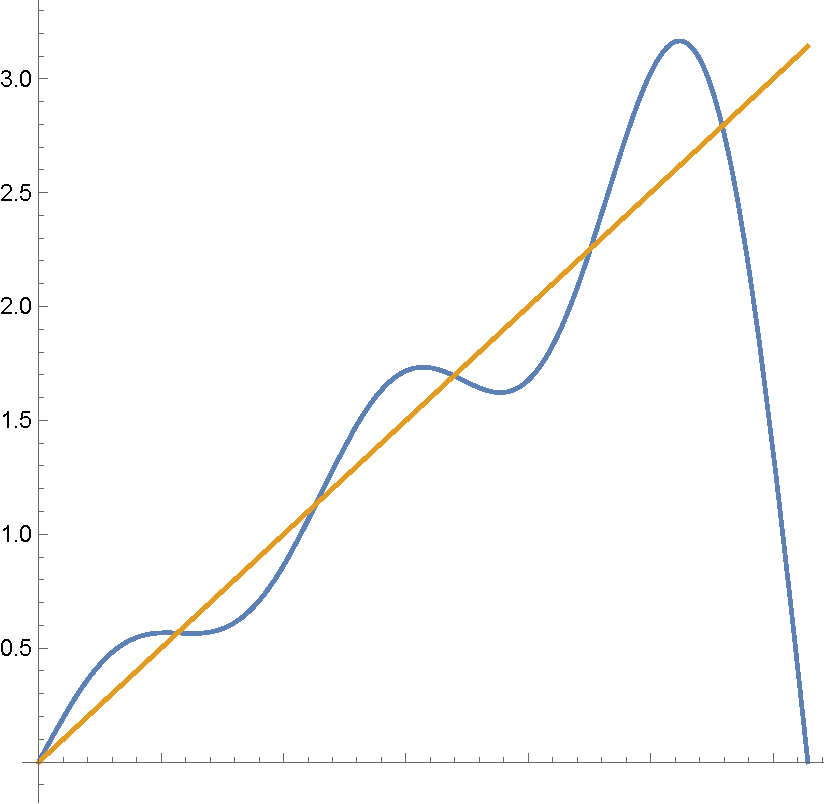
\includegraphics[width=0.5\textwidth]{plots/x-fourier-series-1.pdf}
    \caption{$N = 5$ partial sum of \eqref{eq:4.expansion}}
    \label{fig:partial-sum}
\end{figure}

\section{}

\paragraph*{Problem}  Find the Fourier series of 
\begin{equation}
    f(x)= \begin{cases}-x & \text { for }-5 \leq x<0 \\ 1+x^2 & \text { for } 0 \leq x \leq 5\end{cases}
\end{equation}
and find what it converges to.

\paragraph*{Solution} The Fourier series is 
\begin{equation}
    f(x) = \frac{a_0}{2} 
    + \sum_{n=1}^{\infty} \left(
        a_n \sin(\frac{n \pi x}{5}) + b_n \cos(\frac{n \pi x}{5})
    \right).
\end{equation}
The coefficients are found below. 
For $a_0$ we have 
\begin{equation}
    \begin{aligned}
        a_0 = \frac{1}{5} \int_{-5}^{5} f(x) \dd{x} = \frac{71}{6}.
    \end{aligned}
\end{equation}
When $m \neq 0$,
\begin{equation}
    \begin{aligned}
        a_m &= \frac{1}{5} \int_{-5}^{5} f(x) \cos \frac{m \pi x}{5} \dd{x} \\
        &= \frac{1}{5} \int_{-5}^{0} (-x) \cos \frac{m \pi x}{5} \dd{x}
        + \frac{1}{5} \int_{0}^{5} (x^2 + 1) \cos \frac{m \pi x}{5} \dd{x} \\
        &= \frac{1}{5} \left(\frac{5}{m \pi}\right)^2 
        \int_{0}^{m \pi} x \cos x \dd{x} 
        + \frac{1}{5} \left(\frac{5}{m \pi}\right)^3 
        \int_{0}^{m \pi} x^2 \cos x \dd{x} \\
        &= \frac{1}{5} \left(\frac{5}{m \pi}\right)^2  
        \eval{(x \sin x + \cos x)}_{0}^{m \pi} 
        + \frac{1}{5} \left(\frac{5}{m \pi}\right)^3 
        \eval{(x^2 \sin x + 2 x \cos x - 2 \sin x)}_{0}^{m \pi} \\
        &= \frac{55 (-1)^m - 5}{\pi^2 m^2}.
    \end{aligned}
\end{equation}
The sin coefficients are given by 
\begin{equation}
    \begin{aligned}
        b_m &= \frac{1}{5} \int_{-5}^{0} (-x) \sin \frac{m \pi x}{5} \dd{x}
        + \frac{1}{5} \int_{0}^{5} (x^2 + 1) \sin \frac{m \pi x}{5} \dd{x} \\
        &= - \frac{1}{5} \left(\frac{5}{m \pi}\right)^2
        \int_{0}^{m \pi} x \sin x \dd{x}
        + \frac{1}{5} \left(\frac{5}{m \pi}\right)^3 
        \int_{0}^{m \pi} x^2 \sin x \dd{x} 
        + \frac{1}{5} \frac{5}{m \pi} 
        \int_{0}^{m \pi} \sin x \dd{x} \\
        &= - \frac{1}{5} \left(\frac{5}{m \pi}\right)^2 
        \eval{(-x \cos x + \sin x)}_{0}^{m \pi} 
        + \frac{1}{5} \left(\frac{5}{m \pi}\right)^3 
        \eval{(- x^2 \cos x + 2 x \sin x + 2 \cos x)}_{0}^{m \pi} \\
        &\quad + \frac{1}{5} \frac{5}{m \pi} (- \cos (m \pi) + 1) \\
        &= \frac{ - 21 (-1)^m + 1 }{m \pi} 
        + \frac{50}{m^3 \pi^3} ((-1)^m - 1).
    \end{aligned}
\end{equation}
There is one discontinuity $x = 0$ in $(-5, 5)$.
According to the convergence theorem,
the Fourier series of $f(x)$ converges to $f(x)$ when 
$-5 < x < 0$ or $0 < x < 5$;
it converges to $(f(0^-) + f(0^+)) / 2 = 1 / 2$ at $x = 0$,
and to $(f(-5) + f(5)) / 2 = 31 / 2$ at $x = \pm 5$.

\end{document}